\chapter{Expansion de Friedmann, rayonnement et matière noire}

\section{Rappel de l’équation cosmologique fondamentale}

À des échelles supérieures à celles des amas de galaxies, on considère que l’Univers est homogène. Choisissons les coordonnées de sorte que nous soyons en \(x=0\) et plaçons une galaxie représentative, ou simplement une particule imaginaire entraînée par le flot de Hubble, en \(x=1\). Par définition, sa distance physique par rapport à nous est alors le facteur d’échelle \(a(t)\). Un point situé en \(x=2\) se trouve à la distance \(2a(t)\), et ainsi de suite.

\begin{figure}[ht]
\centering
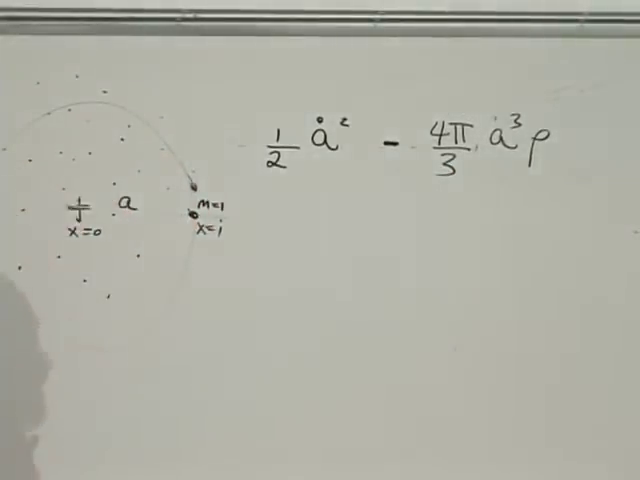
\includegraphics[width=0.78\textwidth]{lecture_03_figure_02.png}
\caption{Sphère homogène centrée en \(x=0\), galaxie comobile en \(x=1\) et bilan énergétique newtonien pour \(a(t)\).}
\end{figure}

Seule la matière contenue dans la sphère de rayon \(a(t)\) contribue à l’attraction gravitationnelle exercée sur la particule située en \(x=1\). Attribuons une masse unité à cette particule. Son énergie cinétique est
\begin{equation}
\frac{1}{2}\dot a^2.
\end{equation}
La masse contenue dans la sphère est
\begin{equation}
M_{\mathrm{enc}}=\frac{4\pi}{3}a^3\rho,
\end{equation}
L’énergie potentielle gravitationnelle est donc
\begin{equation}
-\frac{G M_{\mathrm{enc}}}{a}
=
-\frac{4\pi G}{3}a^2\rho.
\end{equation}
\editorialnote{À l’horodatage 00:05:30 du cours, le tableau montre clairement le terme cinétique et le terme potentiel qui dépend de la densité. Le coefficient complet écrit ici découle de la dérivation orale.}

La conservation de l’énergie donne
\begin{equation}
\frac{1}{2}\dot a^2-\frac{4\pi G}{3}a^2\rho=\text{const}.
\end{equation}
La constante est alors notée \(-k\), avec la mise en garde habituelle : la normalisation standard ne fixe véritablement cette notation qu’après multiplication de l’équation par \(2\). Sous sa forme standard,
\begin{equation}
\dot a^2=\frac{8\pi G}{3}a^2\rho-k,
\end{equation}
et en divisant par \(a^2\), on obtient
\begin{equation}
\left(\frac{\dot a}{a}\right)^2=\frac{8\pi G}{3}\rho-\frac{k}{a^2}.
\end{equation}
C’est l’équation de Friedmann sous la forme utilisée dans toute la discussion.

\begin{figure}[ht]
\centering
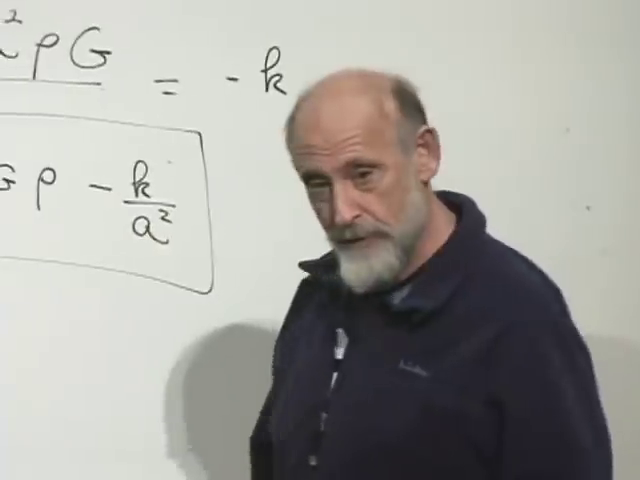
\includegraphics[width=0.56\textwidth]{lecture_03_figure_03.png}
\caption{Contribution de la courbure \(-k/a^2\) isolée dans l’équation de Friedmann.}
\end{figure}

Empiriquement, le terme de courbure est très proche de zéro, au point qu’à ce niveau d’approximation, il est tout à fait justifié de le négliger. Il correspond bien à la courbure de l’espace, mais sa valeur est ici trop faible pour que les observations permettent même d’en déterminer le signe.

La même équation découle aussi de la relativité générale. Sous une forme schématique, l’équation d’Einstein temporelle-temporelle s’écrit
\begin{equation}
R_{00}-\frac{1}{2}g_{00}R \propto T_{00}.
\end{equation}
\editorialnote{La discussion ne donne ici que la structure tensorielle, sans le coefficient numérique global exact.}
Pour une métrique homogène en expansion, le membre géométrique produit la combinaison de \(\dot a/a\) et \(k/a^2\), tandis que le membre de matière donne la densité d’énergie. À ce stade, l’argument newtonien et l’équation d’Einstein expriment la même chose.

Cela modifie aussi le sens de \(\rho\). À partir de maintenant, il vaut mieux appeler \(\rho\) la densité d’énergie. Pour une matière qui se déplace lentement dans le référentiel comobile, il s’agit simplement de la densité d’énergie au repos.

\section{Domination de la matière}

Supposons maintenant que la densité d’énergie soit portée par de la matière au repos dans le référentiel comobile. Considérons un cube d’une unité de coordonnée de côté. Ses côtés physiques mesurent \(a(t)\), et son volume physique est donc \(a^3(t)\). Si l’énergie de masse contenue dans ce cube comobile est \(M\) et que la matière est entraînée par le flot sans traverser ses frontières, alors
\begin{equation}
\rho_m=\frac{M}{a^3}.
\end{equation}

C’est le cas dominé par la matière. Dans cette idéalisation, les particules sont au repos dans la boîte : on prend donc la température et la pression égales à zéro. Une pression supposerait que des particules traversent les frontières de la boîte.

Avec \(k\approx 0\), l’équation devient
\begin{equation}
\left(\frac{\dot a}{a}\right)^2=\frac{8\pi G}{3}\frac{M}{a^3}.
\end{equation}
Essayons une loi de puissance,
\begin{equation}
a(t)=Ct^p.
\end{equation}
Alors
\begin{equation}
\frac{\dot a}{a}=\frac{p}{t},
\end{equation}
Le membre de gauche varie donc comme \(t^{-2}\), tandis que le membre de droite varie comme \(t^{-3p}\). L’égalité des puissances donne
\begin{equation}
3p=2,
\qquad
p=\frac{2}{3}.
\end{equation}
Par conséquent,
\begin{equation}
a(t)\propto t^{2/3}.
\end{equation}
En conservant le coefficient, on obtient
\begin{equation}
C^3=6\pi G M.
\end{equation}

L’essentiel de la solution est la loi de puissance. Un univers dominé par la matière se dilate comme la puissance deux tiers du temps, et non linéairement. Cette loi décrit une longue période intermédiaire, qui commence environ \(10^5\) ans après le Big Bang et s’étend sur quelques milliards d’années. L’Univers actuel n’est pas littéralement dominé par la matière, puisque l’énergie noire domine aujourd’hui, mais la matière ordinaire et une grande partie de l’histoire cosmologique se décrivent ainsi.

\section{Domination du rayonnement}

Plus tôt, la densité d’énergie était dominée par le rayonnement. La raison est simple : l’Univers contient un nombre considérable de photons, environ \(10^9\) photons par proton, et lorsque l’Univers se contracte, ces photons deviennent plus énergétiques.

Un photon n’a pas de masse au repos, mais il possède de l’énergie. Son énergie est
\begin{equation}
E_\gamma=h\nu=\frac{hc}{\lambda}.
\end{equation}
L’hypothèse essentielle est que, lorsque l’Univers se dilate, les longueurs d’onde des photons s’étirent avec lui :
\begin{equation}
\lambda\propto a.
\end{equation}
Une onde dans une boîte donne une bonne image du phénomène. Lorsque la boîte grandit, la longueur d’onde du mode augmente avec elle. On applique ici la même idée à l’expansion de l’Univers.

Puisque \(\lambda\propto a\), l’énergie de chaque photon varie comme
\begin{equation}
E_\gamma\propto a^{-1}.
\end{equation}
Considérons à nouveau une boîte comobile de côté unité. Des photons y entrent et en sortent, mais leur nombre à l’intérieur reste constant en moyenne. L’énergie totale des photons dans la boîte varie alors elle aussi comme \(a^{-1}\). En la divisant par le volume physique \(a^3\), on trouve que la densité d’énergie du rayonnement varie comme
\begin{equation}
\rho_r\propto a^{-4}.
\end{equation}

Ce facteur supplémentaire de \(a^{-1}\) constitue toute la différence. La matière se dilue parce que l’Univers se dilate. Le rayonnement se dilue pour cette même raison, mais aussi parce que chaque photon subit un décalage vers le rouge.

L’équation de Friedmann pour un univers dominé par le rayonnement est donc
\begin{equation}
\left(\frac{\dot a}{a}\right)^2=\frac{8\pi G}{3}\frac{M_r}{a^4}.
\end{equation}
\editorialnote{Dans la discussion orale, le symbole \(M\) est réutilisé pour cette nouvelle constante. L’indice \(r\) est ajouté ici uniquement pour éviter toute confusion avec le cas de la matière.}

Utilisons la même forme d’essai \(a(t)=Ct^p\). Le membre de gauche varie à nouveau comme \(t^{-2}\), tandis que le membre de droite varie comme \(t^{-4p}\). L’égalité des puissances donne
\begin{equation}
4p=2,
\qquad
p=\frac{1}{2}.
\end{equation}
On a donc
\begin{equation}
a(t)\propto t^{1/2}.
\end{equation}
En conservant le coefficient, on obtient
\begin{equation}
C^4=\frac{32\pi G}{3}M_r.
\end{equation}

\begin{classroomqa}
\lecturetimestamp{00:35:41}
\audiencequestion{Pourquoi y a-t-il un \(G\) dans cette équation ?}
\lecturerresponse{Parce que c’est la densité d’énergie, et non la seule masse au repos, qui gravite. Pour la matière en mouvement lent, la distinction est facile à manquer, mais les photons nous l’imposent : ils n’ont pas de masse au repos et gravitent pourtant.}
\end{classroomqa}

Une boîte pleine de rayonnement permet de concrétiser cette idée. Poussons une boîte remplie de photons. Dès que la boîte accélère, la paroi qui avance vers les photons subit des chocs plus intenses que celle qui s’éloigne d’eux ; il faut donc pousser davantage pour vaincre la pression du rayonnement. La boîte possède ainsi une inertie supplémentaire et, selon le principe d’équivalence, cette inertie supplémentaire correspond aussi à une masse gravitationnelle supplémentaire. C’est l’argument de la boîte de photons invoqué ici pour montrer que l’énergie gravite.

\begin{classroomqa}
\lecturetimestamp{00:38:11}
\audiencequestion{L’une ou l’autre de ces équations peut-elle avoir une solution où \(a\) diminue avec le temps ?}
\lecturerresponse{Oui. Si l’on réintroduit le terme de courbure \(k/a^2\), il existe des solutions où l’Univers se dilate, puis se contracte. Ce n’est pas ce que semble faire notre Univers, mais l’équation le permet.}
\end{classroomqa}

\begin{classroomqa}
\lecturetimestamp{00:38:44}
\audiencequestion{Qu’advient-il de la conservation de l’énergie ?}
\lecturerresponse{Si l’on réintroduit le terme \(k\) et que l’on multiplie de nouveau l’équation par \(a^2\), l’équation cosmologique est précisément la loi de conservation. La matière ou le rayonnement d’un côté ne constitue qu’une partie du bilan. L’expansion contribue les termes cinétique et gravitationnel, et le bilan total est conservé.}
\end{classroomqa}

\section{Matière et rayonnement réunis}

En cosmologie réelle, matière et rayonnement sont tous deux présents. Leurs densités varient différemment :
\begin{equation}
\rho_m\propto a^{-3},
\qquad
\rho_r\propto a^{-4}.
\end{equation}
Ainsi, pour de petites valeurs de \(a\), le rayonnement domine. Pour de grandes valeurs de \(a\), c’est la matière qui domine. En remontant le temps, l’Univers primordial devait donc être dominé par le rayonnement.

\begin{figure}[ht]
\centering
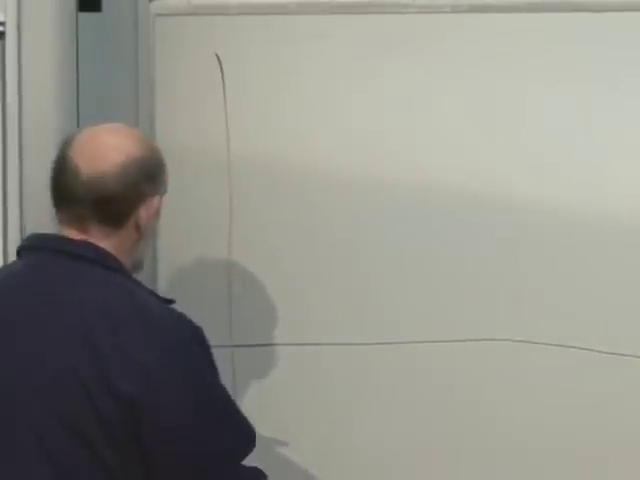
\includegraphics[width=0.68\textwidth]{lecture_03_figure_05.png}
\caption{Axes permettant de comparer les densités d’énergie de la matière et du rayonnement en fonction du facteur d’échelle.}
\end{figure}

\editorialnote{À l’horodatage 00:44:45 du cours, le tableau ne montre que les axes au début du tracé comparatif. Les courbes de la matière et du rayonnement, évoquées juste après, sont décrites dans le texte et ne sont pas représentées à nouveau ici.}

La courbe de la matière décroît comme \(a^{-3}\). Celle du rayonnement décroît comme \(a^{-4}\). Les deux divergent lorsque \(a\to 0\), mais la courbe du rayonnement croît alors plus rapidement ; les deux courbes se croisent donc pour une certaine valeur d’égalité du facteur d’échelle. Selon une estimation approximative, cette transition se produit au bout d’environ \(10^4\) ans, peut-être un peu plus.

On peut exprimer la même idée en traçant \(a(t)\) en fonction de \(t\). Au début, l’expansion suit le comportement \(t^{1/2}\). Plus tard, elle suit le comportement \(t^{2/3}\). Il ne s’agit pas d’un saut, mais d’une transition continue sur une plage de temps relativement étroite.

\begin{classroomqa}
\lecturetimestamp{00:44:04}
\audiencequestion{Avec l’âge de l’Univers, l’exposant \(p\) passe-t-il continûment de \(1/2\) à \(2/3\) ?}
\lecturerresponse{Oui. Il ne change pas brutalement. L’évolution est continue, même si elle se déroule sur une plage de temps assez étroite.}
\end{classroomqa}

\section{Température, recombinaison et dernière diffusion}

La température est la quantité suivante à considérer. Si l’énergie d’un photon typique varie comme \(a^{-1}\), alors il en va de même pour la température du bain de rayonnement :
\begin{equation}
T\propto a^{-1}.
\end{equation}
Si \(a\) double, la température est divisée par deux.

Prenons une température actuelle des photons d’environ \(3\,\mathrm K\) et une température d’ionisation d’environ \(3000\,\mathrm K\), proche de celle de la surface du Soleil. Alors,
\begin{equation}
\frac{a_{\mathrm{today}}}{a_{\mathrm{ion}}}\sim 10^3.
\end{equation}
En utilisant la loi de domination tardive de la matière \(a\propto t^{2/3}\),
\begin{equation}
\left(\frac{t_{\mathrm{today}}}{t_{\mathrm{ion}}}\right)^{2/3}\sim 10^3,
\end{equation}
on obtient
\begin{equation}
\frac{t_{\mathrm{today}}}{t_{\mathrm{ion}}}\sim 1000^{3/2}\sim 3\times 10^4.
\end{equation}
En prenant, pour cette estimation, l’âge de l’Univers égal à \(10^{10}\) ans, on trouve
\begin{equation}
t_{\mathrm{ion}}\sim 3\times 10^5\ \mathrm{years}.
\end{equation}

C’est l’époque à laquelle l’hydrogène et l’hélium cessent d’être entièrement ionisés. Avant cela, l’Univers est un plasma chaud. Pourquoi un plasma est-il opaque ? Parce que les charges libres réagissent fortement aux ondes électromagnétiques. Le champ électrique entraîne les charges dans un mouvement de va-et-vient ; le milieu se comporte comme un conducteur, et les conducteurs sont opaques. C’est l’analogie pertinente avec la surface du Soleil.

Lorsque l’Univers se refroidit suffisamment pour que les électrons se recombinent avec les noyaux, des atomes neutres ordinaires se forment et l’Univers devient beaucoup plus transparent. La transition n’est pas infiniment abrupte. Elle se produit dans une zone floue, ou sur un intervalle de temps flou, mais elle est suffisamment nette en cosmologie pour qu’on l’appelle la surface de dernière diffusion.

Observer au loin revient à regarder dans le passé. Les galaxies proches nous montrent le passé récent. Les galaxies plus lointaines révèlent des époques antérieures. À une distance suffisante, chaque ligne de visée atteint l’époque où l’Univers était encore ionisé et opaque. Le rayonnement électromagnétique ne peut rien nous montrer d’antérieur.

En principe, d’autres messagers pourraient sonder des époques plus anciennes. Les neutrinos, électriquement neutres, se découpleraient plus tôt. Les gravitons, si l’on pouvait un jour les observer, proviendraient d’époques encore plus anciennes. Mais la même faiblesse d’interaction qui leur permettrait de traverser le plasma primordial les rend aussi extrêmement difficiles à détecter.

Si l’Univers a jadis été aussi chaud que la surface du Soleil dans toutes les directions, pourquoi le ciel n’est-il pas d’un éclat aveuglant ? Parce que la surface de dernière diffusion s’éloigne et que les photons qui nous en parviennent ont subi un décalage vers le rouge d’un facteur d’environ \(10^3\), correspondant à l’écart entre \(3000\,\mathrm K\) et \(3\,\mathrm K\). Ce qui nous parvient est un rayonnement micro-onde, et non de la lumière visible du Soleil.

\begin{classroomqa}
\lecturetimestamp{01:03:51}
\audiencequestion{Nos télescopes ne peuvent donc pas regarder au-delà d’environ \(300{,}000\) ans ?}
\lecturerresponse{Les télescopes électromagnétiques ne le peuvent pas. Avant cette époque, l’Univers était ionisé et opaque. D’autres messagers pourraient, en principe du moins, sonder des époques antérieures.}
\end{classroomqa}

\begin{classroomqa}
\lecturetimestamp{01:08:43}
\audiencequestion{Quand vous parlez de la température d’un photon, vous voulez dire la température d’un corps noir dont le rayonnement a ce maximum. Mais cette relation n’est pas linéaire en fonction de la longueur d’onde, n’est-ce pas ?}
\lecturerresponse{C’est exact. La température correspond essentiellement à l’énergie d’un photon typique ; pour un photon, elle varie donc en raison inverse de la longueur d’onde. La loi \(T^4\) se rapporte à la densité d’énergie, et non à l’énergie d’un photon individuel. Elle combine l’énergie par photon et le nombre de photons par unité de volume, la densité numérique variant comme \(T^3\).}
\end{classroomqa}

On a donc
\begin{equation}
n_\gamma\propto T^3,
\qquad
\rho_\gamma\propto T^4.
\end{equation}

\section{La matière noire révélée par les courbes de rotation}

La matière noire intervient dans l’étude des courbes de rotation galactiques. Elle n’a pas été déduite de l’équation de Friedmann à grande échelle, mais des observations astronomiques à l’échelle des galaxies.

Commençons par le problème newtonien le plus simple : un petit corps de masse \(m\) en orbite autour d’une masse centrale \(M\) à la distance \(r\). La force gravitationnelle vaut
\begin{equation}
\frac{GMm}{r^2},
\end{equation}
et l’accélération centripète est \(v^2/r\). La loi de Newton donne
\begin{equation}
m\frac{v^2}{r}=\frac{GMm}{r^2}.
\end{equation}
Simplifions par \(m\), multiplions par \(r\) et obtenons
\begin{equation}
v(r)=\sqrt{\frac{GM}{r}}.
\end{equation}
Ainsi, si la masse gravitationnelle est concentrée près du centre, la vitesse orbitale décroît comme \(r^{-1/2}\).

C’est ce à quoi l’on s’attendrait si la masse suivait la lumière. La majeure partie de la matière visible d’une galaxie se trouve près de son noyau ; les étoiles extérieures se comporteraient alors un peu comme les planètes éloignées du système solaire. Les astronomes déduisent les vitesses orbitales en mesurant les différences de décalage Doppler de part et d’autre d’une galaxie proche : ils comparent le côté qui se rapproche de nous à celui qui s’en éloigne, après avoir soustrait le mouvement global de récession de la galaxie. Les vitesses orbitales mesurées restent à peu près constantes jusqu’à de grands rayons.

Remplaçons donc la masse centrale \(M\) par la masse intérieure \(M(r)\) :
\begin{equation}
\frac{v^2}{r}=\frac{G M(r)}{r^2}.
\end{equation}
Si \(v(r)\) est approximativement constante, alors
\begin{equation}
M(r)\propto r.
\end{equation}
Autrement dit, la masse gravitationnelle continue d’augmenter avec le rayon, même là où la lumière visible n’augmente pas.

Supposons maintenant, comme le fait la discussion par souci de simplicité, que la distribution de masse soit à peu près sphérique. Alors,
\begin{equation}
M(R)=\int_0^R 4\pi r^2\rho(r)\,dr.
\end{equation}
Si \(M(R)\propto R\), la dérivation par rapport à \(R\) donne
\begin{equation}
4\pi R^2\rho(R)\propto 1,
\end{equation}
et par conséquent
\begin{equation}
\rho(r)\propto \frac{1}{r^2}.
\end{equation}

\begin{classroomqa}
\lecturetimestamp{01:28:18}
\audiencequestion{La densité devrait varier comme \(1/r^2\), semble-t-il. Y a-t-il une raison à cela ?}
\lecturerresponse{À partir de la courbe de rotation plate observée, on déduit \(M(R)\propto R\), puis la dérivation donne \(\rho(r)\propto 1/r^2\). On ne prétend pas aller plus loin ici dans l’explication à partir de principes premiers ; les simulations détaillées font une grande partie du travail.}
\end{classroomqa}

La conclusion solide est qu’une galaxie contient beaucoup plus de masse gravitationnelle que ne le laisserait supposer la seule matière lumineuse : plusieurs fois plus, et environ un ordre de grandeur de plus selon l’estimation utilisée ici. La galaxie visible se trouve à l’intérieur d’un halo sombre bien plus étendu.

Qu’est-ce qui empêche le gaz ordinaire de rester aussi diffus ? La dissipation. Un nuage de gaz se contracte parce que les collisions, les processus analogues au frottement et le rayonnement lui permettent de perdre de l’énergie. La matière noire ne rayonne manifestement pas de façon appréciable et est presque sans collisions. La gravité peut l’attirer vers l’intérieur et convertir l’énergie potentielle en énergie cinétique, mais, faute d’une dissipation efficace, elle ne s’effondre pas pour former les structures lumineuses compactes que produit la matière ordinaire. C’est l’énergie cinétique qui maintient le halo étendu.

Plusieurs autres possibilités sont alors évoquées avec prudence. Il est dit que les neutrinos sont trop rapides pour se comporter ainsi à l’échelle des galaxies. Un halo constitué d’hydrogène ordinaire perturberait fortement la nucléosynthèse de l’Univers primordial. Les trous noirs formés de matière ordinaire sont également mentionnés comme une possibilité problématique : ils impliqueraient une quantité excessive de matière ordinaire dans l’Univers primordial et soulèveraient des questions de lentillage gravitationnel. La discussion n’affirme rien de plus à ce stade.

Le halo n’est pas décrit comme une coquille mince ni comme un tore. C’est une sphère approximative et non uniforme, plus dense vers le centre et dont la densité diminue progressivement vers l’extérieur.

\begin{classroomqa}
\lecturetimestamp{01:53:12}
\audiencequestion{Parlez-vous de l’amas du Boulet ?}
\lecturerresponse{Oui. Le gaz observé en rayons X révèle la matière ordinaire, tandis que le lentillage révèle la masse gravitationnelle totale. Lors de la collision, ces deux distributions se séparent. C’est un argument solide en faveur de l’existence réelle de matière noire, plutôt que d’une simple modification de la gravité liée uniquement à la matière visible.}
\end{classroomqa}

C’est le dernier point observationnel. On sait peu de choses en détail sur la nature de la matière noire, mais rien de ce qui précède n’exige un principe radicalement nouveau. L’hypothèse prudente est simplement que la nature contient des particules supplémentaires, interagissant faiblement, qui n’ont pas encore été identifiées.
